%!TEX root = ../doc.tex
\chapter{Testing and Results}
\label{sec:Results}
The following chapter describes the calibration, testing and the results of the system components. 
\section{ToF Camera}
The time-of-flight camera is the crucial part of this thesis, allowing a three-dimensional scene reconstruction. This section describes the measurements and the results of the motion estimation of the ToF Camera at every involved step.
\subsection{Setup}
As described in section \ref{sec:camHead}, the ToF camera sends its data by ethernet, using a lightweight TCP protocol. The software controlling the setup of the ToF camera runs on the Raspberry Pi and is the proprietary part of the ToF software stack. The software allows a basic configuration in two main modes: automatic and manual control. The software supports HDR functionality in both automatic and manual control, which significantly enhances the dynamic range on the infrared black-and-white image. The implementation of the HDR function is not documented by the supplier of the Nimbus 3D ToF camera.\\ 
The ToF camera uses an infrared flash, which is not brightness-controlled; setting the camera to a fixed exposure time would lead to overexposure on close objects. The automatic mode lets the user select a maximum amplitude of the image, to which the exposure time is set. As the CudaSift library, which extracts the SIFT features from the ToF camera, only supports the 8-bit resolution, the maximum amplitude got selected at 255. Higher values lead to a longer exposure time and let the frame rate drop. Not needing any amplitude scaling while keeping a high frame rate is favorable. 
\begin{figure}[H]
    \centering
    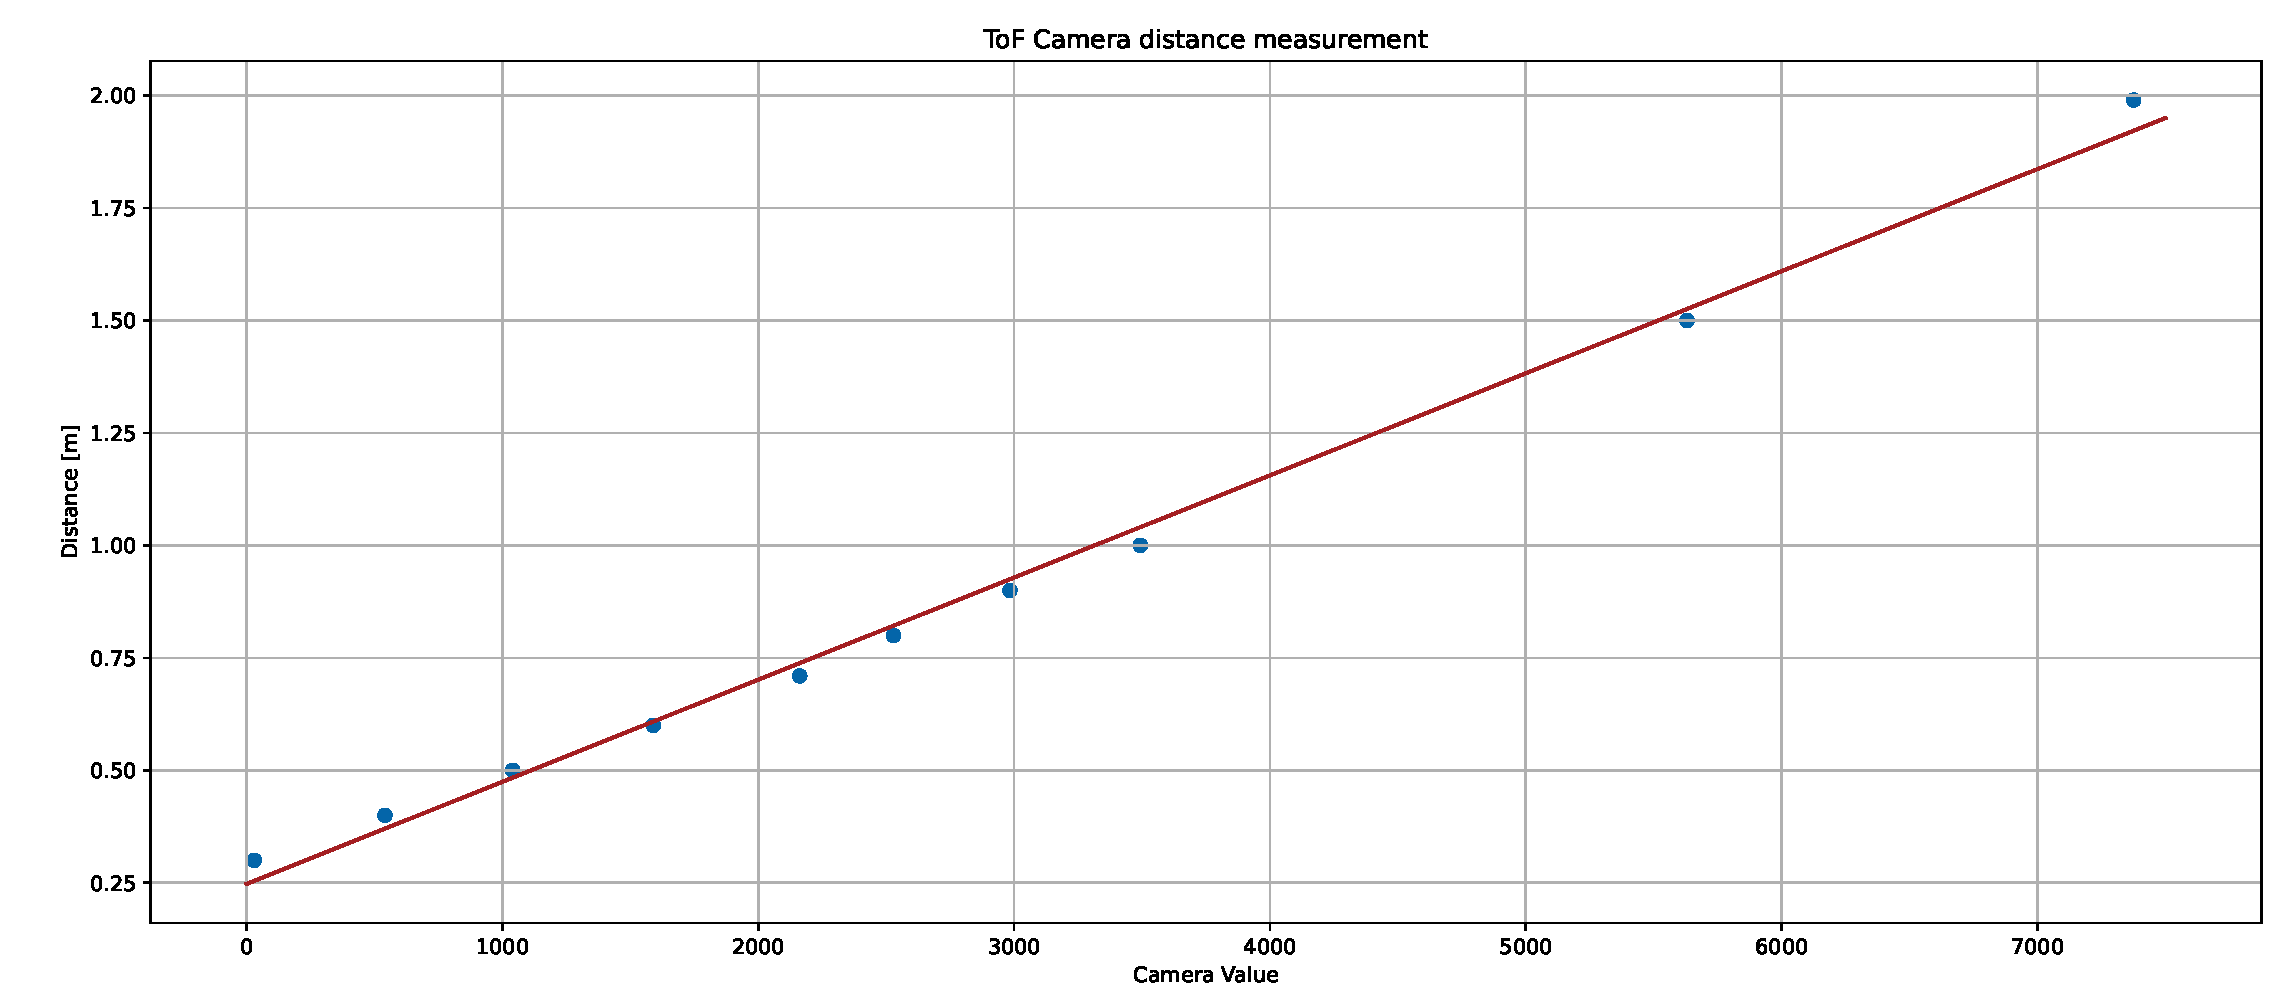
\includegraphics[width=1.0\textwidth]{images/camera_distance_measurement.eps}
    \caption{Sensor values measured against a meterstick. In red, the linear fit generated in Microsoft Excel.}
    \label{im:distance_measurement}
\end{figure}
The coordinate system is not corrected for $x$, $y$ and $z$ yet, as the ToF camera itself does not know its rotation in the field of gravity. Therefore, the axis for the ToF camera calculations are kept in the $a$, $b$ and $c$ system. Details are explained in section \ref{sec:ABC_XYZ_coords}.
\subsection{Distance measurement}
\label{sec:results_distance_meas}
Every pixel of a ToF camera sensor combined with the wide-area infrared flash acts like a laser rangefinder. A single pixel of the sensor targeting a brown cardboard surface positioned at various distances allows measuring this distance with a meterstick and a comparison with the sensor pixel value. A linear fit in Microsoft Excel leads to the following function, which is also visualized in image \ref{im:distance_measurement}:
\begin{equation*}
    d [m] = 0.000227 * val +0.247532
\end{equation*}
The camera noise does affect not only the black-and-white image but also the distance measurement. At the chosen camera settings, the camera noise lets the distance measurement have a standard deviation of around 7mm in the $a$-axis.\\
The formulae for the 3D scene reconstruction propagate the standard deviation to about 4mm in the $b$-axis and 3mm in the $c$-axis.
\subsection{3D Scene Reconstruction}
After calibrating the lens and correcting the radial nature of the distance measurement as described in section \ref{sec:ToFCalibration}, the generated point cloud should directly reconstruct the three-dimensional scene recorded by the ToF camera. Section \ref{sec:ToFPosition_SIFT} describes the process of this reconstruction.
Straight lines in the real world should appear straight in the point cloud, which can be checked by analyzing an image. The two images in figure \ref{fig:linearity3d} demonstrate the point cloud generation, by mapping SIFT features into the 3D space. 
\begin{figure}[H]
    \centering
    \begin{minipage}[b]{0.45\textwidth}
      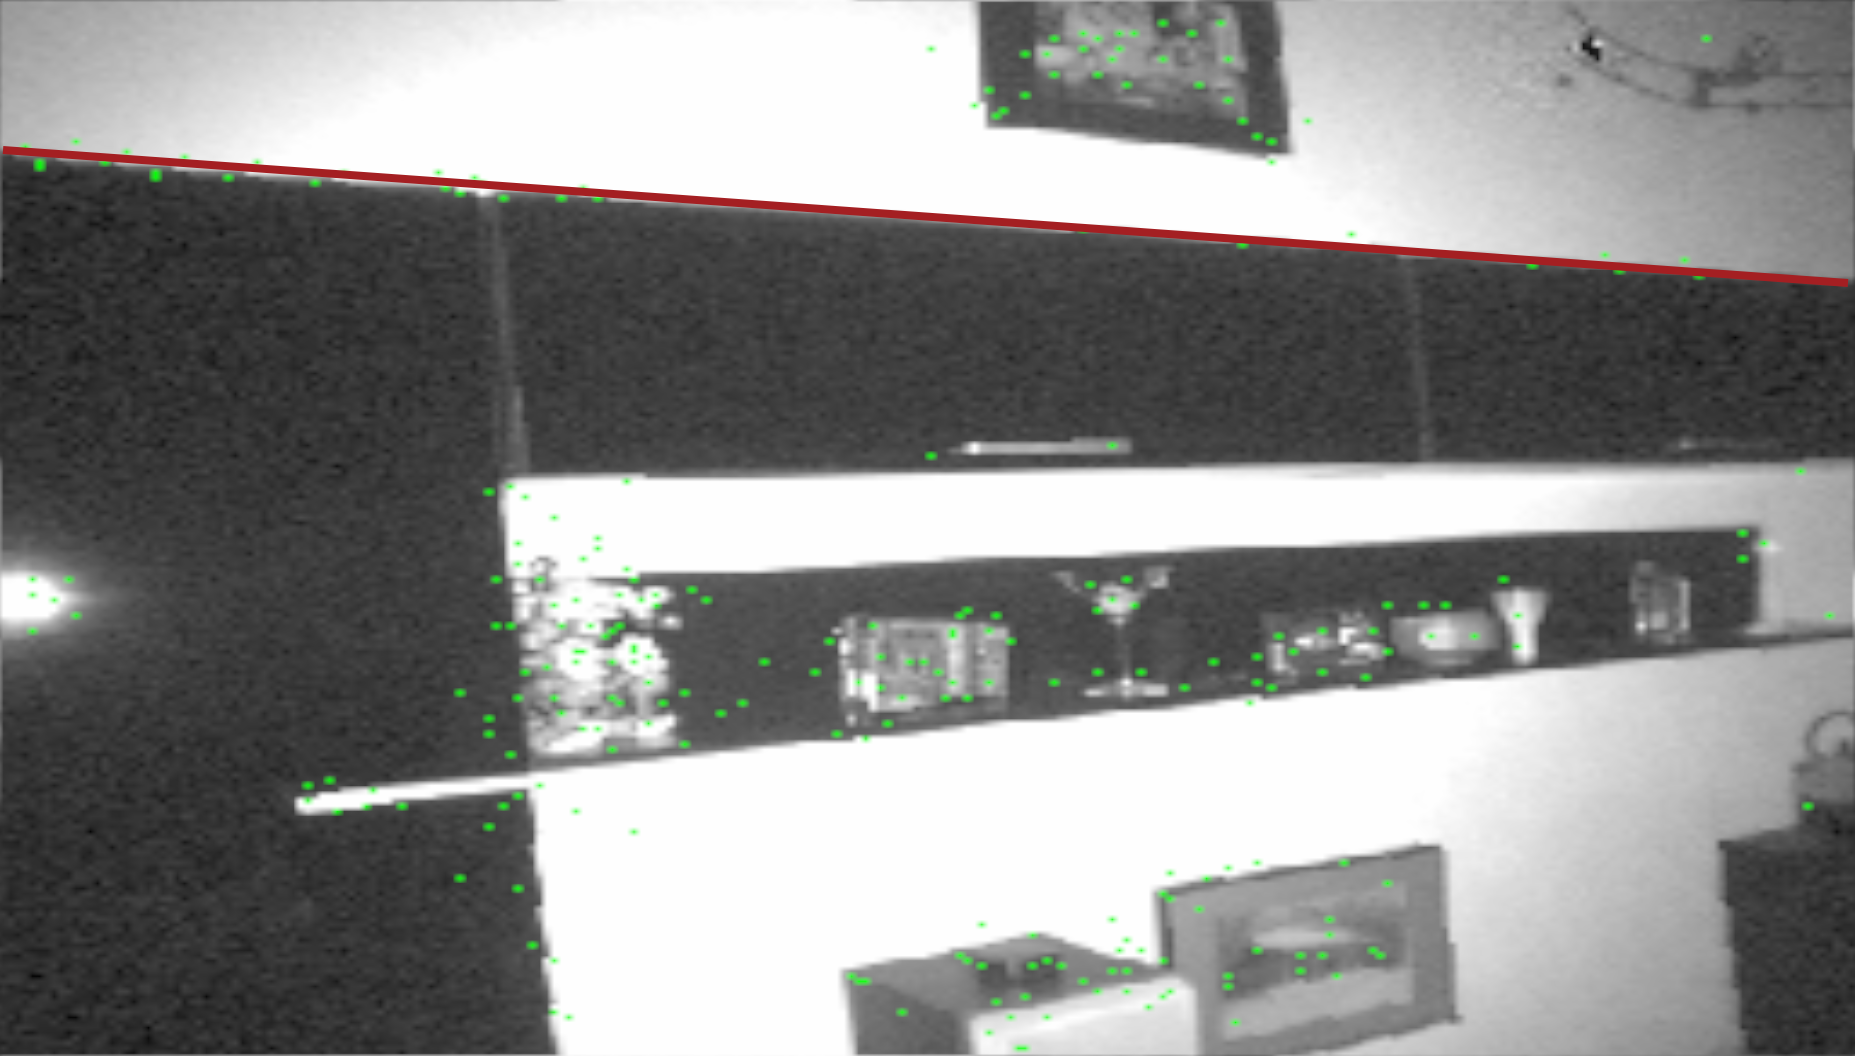
\includegraphics[scale=0.105]{images/cloud_3d_linearity_image.png}
      \caption{Image}
      \label{fig:linearity3d_image} 
    \end{minipage} % Hier darf keine Leerzeile zwischen den beiden Minipages liegen!
    \begin{minipage}[b]{0.45\textwidth}
      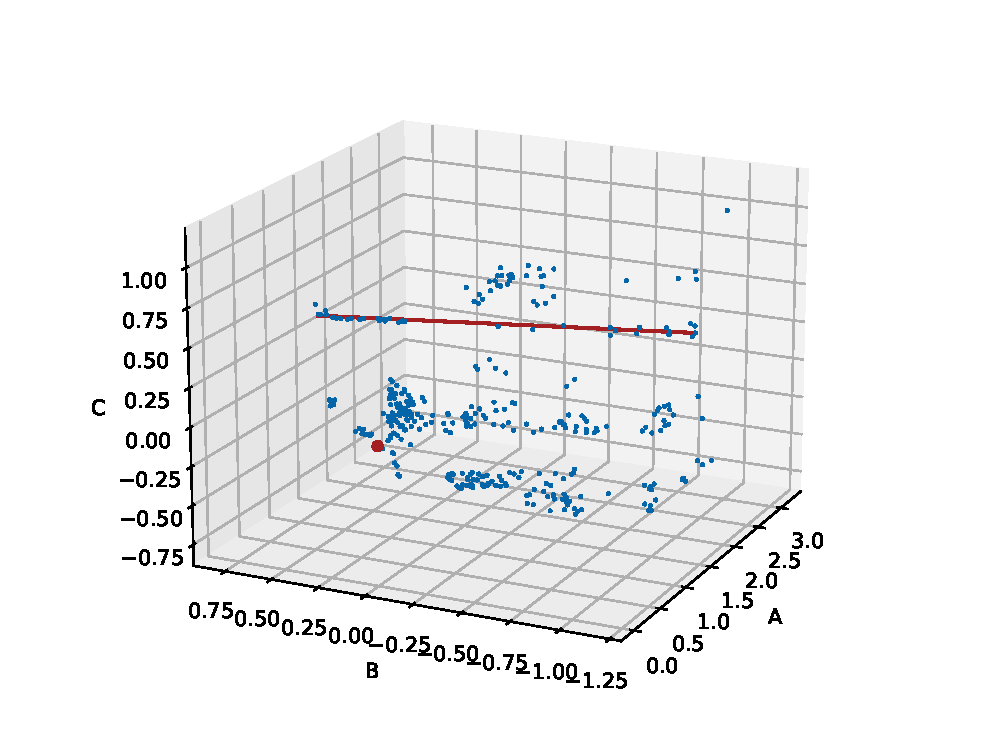
\includegraphics[scale=0.40]{images/linearity_3d.eps} 
      \caption{Cloud}
      \label{fig:linearity3d_cloud} 
    \end{minipage}
    \caption{The scene reconstruction from the left image to the full point cloud. The red line is equivalent in both figures. Each green dot in the image on the left is a SIFT feature. The red dot in the point cloud is the position of the camera.}
    \label{fig:linearity3d}
  \end{figure}
\subsection{RANSAC feature matching}
\label{sec:RANSAC_Results}
The RANSAC algorithm improves the quality of matched features over the flawed brute-force matcher. Section \ref{sec:ToFPosition_RANSAC} explains the implementation of the three-dimensional RANSAC and mentions a threshold. The noisy data the ToF camera delivers gives single SIFT features a positional uncertainty. As discussed in section \ref{sec:results_distance_meas}, the standard deviation in the $a$-axis is roughly 7mm, which also affects the mapping to the$b$- and $c$-axis from the 3d reconstruction. Therefore, the RANSAC matcher is required to have flexibility against positional noise.\\
Prior analysis of the dataset tells a possible rotation and translation. This rigid motion moves each data point in the old cloud to an estimated position, where a data point of the new cloud is expected.  The lowest sum of square differences (SSD) of all the possible matches to the estimated position determines a match. It is accepted if this matched point lies inside the chosen SSD threshold. 
The SSD creates a sphere around the estimated position. The equation of a sphere of radius $r$ follows the equation $r^{2}=x^{2}+y^{2}+z^{2}$. Setting the radius $r$ equal to the standard deviation of 7 mm on the $a$-axis results in a threshold of around 0.00005. Statistically, around 68\% of the matches should reside inside this sphere of 14 mm diameter. The error on the other axis is smaller as discussed in section \ref{sec:results_distance_meas}, this does not explain the poor matching performance at this threshold, as seen in image \ref{im:noise_against_thresh}. Because of the image noise on the black-and-white image, the extracted SIFT features jitter. Even a jitter in the range of 1 pixel easily leads - depending on its distance - to an error of more than a centimeter. On the other hand, to detect a lateral speed of 0.1 m/s at a frame rate of approximately 10 frames per second, a shift of 1 cm needs to be detected.
\begin{figure}[H]
    \centering
    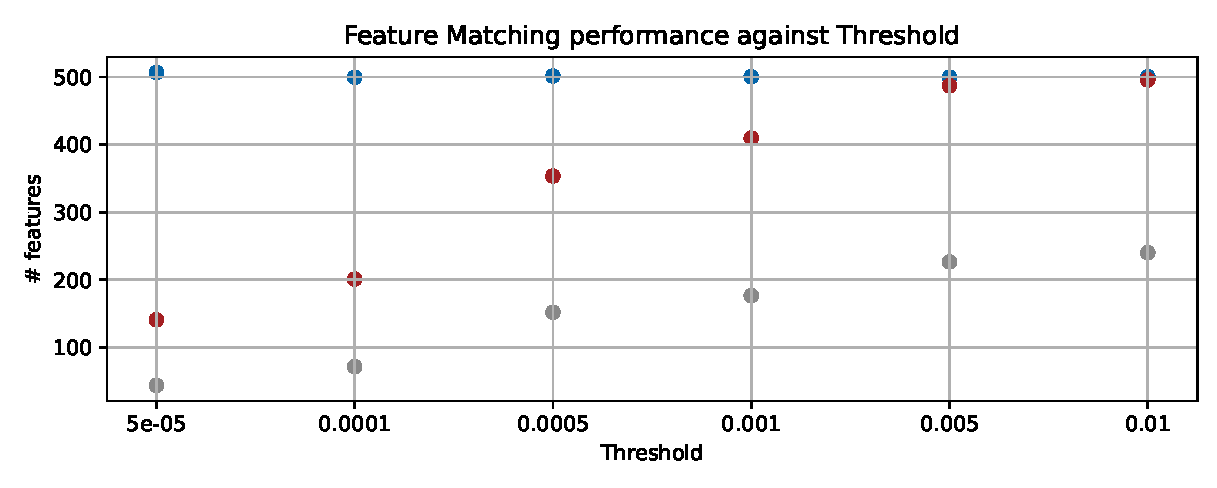
\includegraphics[width=1.0\textwidth]{images/noise_against_threshold.eps}
    \caption{Plotting the feature matching performance against different thresholds shows the quality of the RANSAC feature matcher. In blue, the raw number of unmatched features in each test, in gray the brute force matches and in red the RANSAC matches.}
    \label{im:noise_against_thresh}
\end{figure}
Higher tresholds in image \ref{im:noise_against_thresh} show the expected performance of the brute-force matcher in grey, which lies below 50\% according to the developers of the CudaSift library.\cite{cudaSiftRepo} The RANSAC feature detector vastly improves the matching performance, seemingly up to over 97\% at the threshold of 0.005. At the threshold of 0.005, the sphere around the expected position measures over 14 cm in diameter. The RANSAC matcher might find the same match for different feature points; its matches are not exclusive, combined with the large threshold, it is likely that most features find a match.\\
The balance between the uncertainty and the requirements for detecting slow speeds lead to a chosen threshold of 0.0005.
\subsection{Mapping between RaspiCam and 3D space}
TODO
\section{ToF Rotation}
TODO
\section{ToF Translation}
TODO
\section{Fusion with Kalman Filter}
